% Shared by the three variants (% Shared by the three variants (% Shared by the three variants (% Shared by the three variants (\input{controls} / \input{../controls}); numbers from results/robomme/paired_tests.txt.
\providecommand{\ctrlroot}{}
\section{Matched Controls}
\label{app:controls}

All cells in this section use the released FrameSamp-Modul checkpoint on the test split, $n{=}50$ episodes on the seeds, scenes and distractors of the main tables. Differences are paired, with Bonett--Price 95\% intervals and exact McNemar $p$-values.

\begin{figure}[h]
\centering
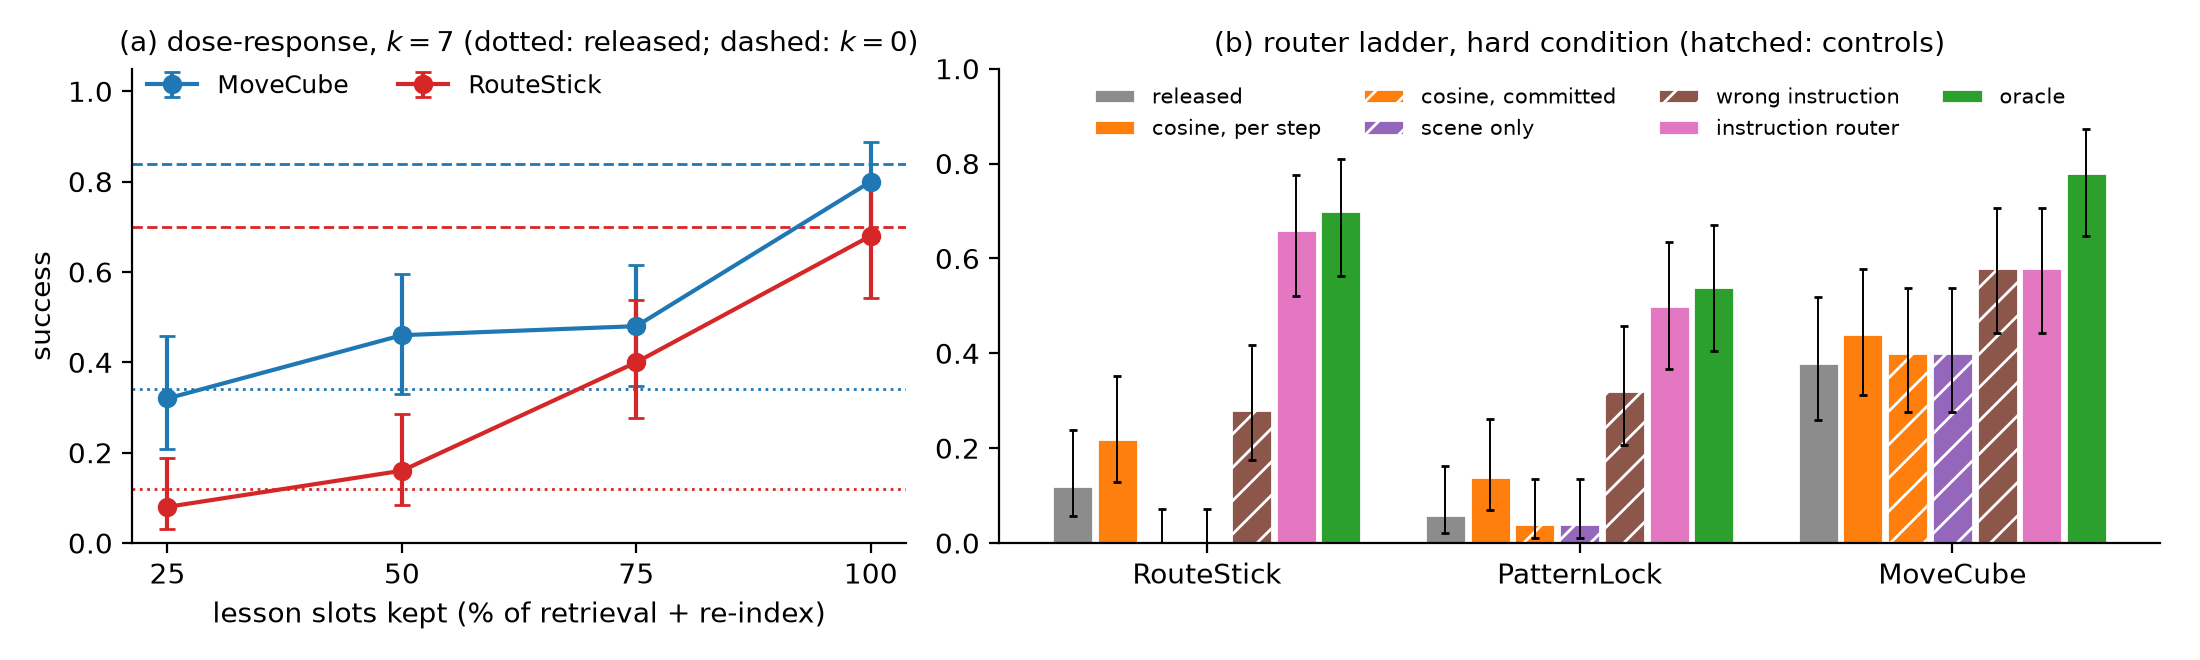
\includegraphics[width=\linewidth]{fig/controls.png}
\caption{(a)~Allocation dose-response on retrieval + re-index's own layout at $k{=}7$: success against the fraction of its lesson slots kept, the freed slots given to distractor frames (100\%: retrieval + re-index). (b)~Router ladder in the hard condition (Table~\ref{tab:ladder}). Wilson 95\% intervals, $n{=}50$ per cell.}
\label{fig:controls}
\end{figure}

\textbf{Router ladder (hard condition).} Three controls separate the parts of the instruction router. \sys{cosine, committed}: the policy-feature cosine retrieval of the main text, deciding once per episode. \sys{scene only}: the router's own encoder, gate and single decision, choosing the session most similar to the current view and never reading the instruction. \sys{wrong instruction}: the full router given the instruction of another task family, fixed per episode. Table~\ref{tab:ladder}: commitment and the encoder contribute nothing by themselves; both committed appearance routers choose a same-scene replay in every episode on all three tasks and score at or below per-step cosine retrieval (RouteStick $.22\to.00$, $p=.001$). The correct instruction is worth $+.38$ $[.22,.51]$ over the wrong one on RouteStick ($p=4\times10^{-6}$) and $+.18$ $[.02,.33]$ on PatternLock ($p=.049$). On MoveCube it is worth nothing ($.58$ vs $.58$, eight discordant episodes each way): the router's gain over the released model there does not come from reading the instruction. A wrong instruction still beats the released model on PatternLock ($+.26$, $p=.002$) and MoveCube ($+.20$, $p=.02$), because any text query breaks the appearance tie among the same-scene sessions and lands on the lesson in $.37$--$.41$ of the slots.

\begin{table}[h]
\centering\small
\caption{Router ladder, hard condition ($k{=}7$, three same-scene replays, $n{=}50$). The three middle columns are the controls; routed systems are re-indexed.}
\label{tab:ladder}
\setlength{\tabcolsep}{5pt}
\begin{tabular}{lccccccc}
\toprule
 & & cosine, & cosine, & scene & wrong & instruction & \\
task & released & per step & committed & only & instruction & router & oracle\\
\midrule
RouteStick & .12 & .22 & .00 & .00 & .28 & .66 & .70\\
PatternLock & .06 & .14 & .04 & .04 & .32 & .50 & .54\\
MoveCube & .38 & .44 & .40 & .40 & .58 & .58 & .78\\
\bottomrule
\end{tabular}
\end{table}

\textbf{Comb isolation.} At $k{=}0$ we keep the released sampler's lesson frames and their number and change only how the current-episode slots are laid out: the most recent frames densely, or every fourth frame back from the present (Table~\ref{tab:comb}). The dense window costs $.50$ $[.33,.64]$ on MoveCube ($p=4\times10^{-7}$) and $.16$ $[.02,.29]$ on VideoPlaceButton ($p=.04$), and its episodes run to the time limit; stride four is within $.10$ $[-.03,.22]$ and $.02$ $[-.09,.13]$ of the released layout. The policy needs its own episode spread over time; it does not need the exact even comb.

\begin{table}[h]
\centering\small
\caption{Left: comb isolation at $k{=}0$ (lesson frames and counts identical in all three columns). Right: index magnitude against relative gap, MoveCube at $k{=}0$ with the released frames (only positions change).}
\label{tab:comb}
\setlength{\tabcolsep}{5pt}
\begin{tabular}{lccc}
\toprule
task & released (even) & stride 4 & dense recent\\
\midrule
MoveCube & .84 & .74 & .34\\
VideoPlaceButton & .58 & .56 & .42\\
\bottomrule
\end{tabular}\qquad
\begin{tabular}{lc}
\toprule
positions & MoveCube\\
\midrule
trained layout & .84\\
current episode $+480$ & .62\\
every frame $+480$ (gap kept) & .68\\
\bottomrule
\end{tabular}
\end{table}

\textbf{Index magnitude or relative gap.} Moving only the current episode's positions 480 steps later costs $.22$ $[.07,.36]$ on MoveCube ($p=.007$). Moving \emph{every} position 480 steps later, which keeps the gap between lesson and episode at its trained value, costs $.16$ $[.03,.28]$ ($p=.02$), and the two do not differ ($+.06$ $[-.08,.19]$). The loss follows the absolute index, not the gap, which is why compacting to the trained range is the fix.

\textbf{Session boundaries.} The managers are given session boundaries. On RouteStick in the hard condition, merging the lesson with its neighbouring session leaves the instruction router unchanged ($.64$ vs $.66$, $-.02$ $[-.13,.09]$). Splitting the lesson at its midpoint is fatal ($.08$, $p=3\times10^{-8}$): the router commits to one half and the policy sees half a route. A deployed segmenter should err towards coarse sessions.

\textbf{Allocation dose-response.} At $k{=}7$ on the standard protocol we fix the number of slots given to the lesson, the current episode and the distractor sessions (Table~\ref{tab:dose}). Success rises with the lesson's slots on both tasks (8 to 24 slots: MoveCube $+.22$, $p=.013$; RouteStick $+.34$, $p=8\times10^{-5}$), and re-indexing changes no cell (all paired differences within $.06$). With eight or fewer lesson slots the policy is at its no-lesson floor. The lesson count is not sufficient, however: with 24 lesson slots, no distractor frame in memory and trained positions, both tasks remain below retrieval + re-index (MoveCube $-.28$, $p=.013$; RouteStick $-.24$, $p=.004$), whose only difference is that the current episode's share grows with the episode instead of staying at eight slots. On RouteStick an even subset of 24 lesson frames beats a random subset of 24 ($.48$ vs $.30$, $p=.004$); at 16 slots the two do not differ. A last series varies the share on a schedule that does reach the reference: retrieval + re-index's own comb over lesson and current episode, with only 25, 50 or 75\% of its lesson slots kept and the freed slots given to distractor frames (lesson share $.2$, $.4$, $.55$; reference $.87$--$.89$). Success is monotone in the fraction kept on both tasks (Fig.~\ref{fig:controls}a), MoveCube $.32/.46/.48/.80$ and RouteStick $.08/.16/.40/.68$ at $25/50/75/100\%$ ($25$ vs $100\%$: $+.48$ $[.29,.63]$, $p=8\times10^{-6}$, and $+.60$ $[.43,.72]$, $p=2\times10^{-9}$), and at 25\% it equals the released model ($-.02$, $-.04$). The curve is convex: giving up the last quarter of the lesson's slots costs $.32$ $[.13,.48]$ and $.28$ $[.12,.42]$ ($p=.002$, $.001$), about what the fixed 24-slot cells lose with no distractor frame in memory. The slot share of Fig.~\ref{fig:mechanism} is therefore causal on the trained layout and steep near the top: the policy needs close to the whole lesson comb, and a partial share buys less than its proportion.

\begin{table}[h]
\centering\small
\caption{Allocation dose-response, standard protocol, $k{=}7$: success by slots given to the lesson / current episode / distractor sessions (32 in total). Upper rows at recorded positions, lower rows re-indexed. 24r: a random instead of an even subset of 24 lesson frames. Reference: retrieval + re-index, which gives every history slot to the lesson and lets the current episode's share grow.}
\label{tab:dose}
\setlength{\tabcolsep}{3pt}
\begin{tabular}{lccccccccc|c}
\toprule
lesson/episode/distr. & 0/16/16 & 4/16/12 & 8/16/8 & 12/16/4 & 16/16/0 & 16/8/8 & 20/8/4 & 24/8/0 & 24r/8/0 & ref.\\
\midrule
MoveCube & .40 & .36 & .36 & .38 & .38 & .42 & .32 & .50 & .46 & .80\\
RouteStick & .10 & .10 & .06 & .14 & .38 & .36 & .52 & .48 & .30 & .68\\
\midrule
MoveCube, re-indexed & & & .30 & & .44 & & & .52 & & .80\\
RouteStick, re-indexed & & & .10 & & .38 & & & .44 & & .68\\
\bottomrule
\end{tabular}
\end{table}

\textbf{Same-task competitors.} The hard condition's replays are motions of other task families. In a stricter variant the three same-scene sessions replay other recorded episodes of the \emph{same} task (another cube target) in the query scene. On MoveCube: released $.32$, cosine retrieval + re-index $.42$, instruction router $.48$, lesson oracle + re-index $.82$ ($k{=}0$: $.84$; oracle against $k{=}0$ $-.02$ $[-.12,.08]$). The router is not better than cosine retrieval ($+.06$ $[-.13,.25]$) and is far below the oracle ($p=8\times10^{-5}$). Offline, scene-plus-instruction routing picks the lesson in $.46$ of MoveCube and $.64$ of RouteStick scenes (chance $.25$; scene-only $.00$): the instruction is the same for every competitor, and what remains is that the lesson is a video and the competitors are robot replays. RouteStick closed loop gives the same picture: released $.18$, cosine retrieval + re-index $.30$, instruction router $.44$, oracle $.68$ ($k{=}0$: $.70$; $-.02$ $[-.08,.05]$); the router beats the released model ($+.26$ $[.07,.43]$, $p=.011$) but not cosine retrieval ($+.14$ $[-.05,.32]$) and is below the oracle ($p=5\times10^{-4}$). Learned routers were never trained on such competitors; applied unchanged, the in-task router of \S\ref{sec:hard} transfers on MoveCube ($.74$, 41 of 50 episodes routed to the lesson; $-.08$ $[-.19,.04]$ against the oracle, $+.26$ $[.08,.42]$ over the instruction router, $p=.007$) and not on RouteStick (in-task $.34$, 26 of 50; leave-one-task-out $.20$, 12 of 50; both below the oracle, $p\le8\times10^{-5}$). Allocation still recovers the no-interference level when the lesson is found; none of our label-free routers finds it reliably among same-task sessions, and a label-trained one does so on one task of two. We note that these replays start from the reset query state, so ``the session least like the current view'' would identify the lesson in every episode; we do not use this cue, which is a property of the construction.

\textbf{What a router sees.} Fig.~\ref{fig:qual} shows the sessions of one test episode per task (episode 3 of each, chosen without reference to outcomes) as the evaluator stores them. The unrelated session of the standard protocol is in another scene, so any similarity to the current view rejects it. A replay recorded in the query scene begins at the current view itself, so cosine retrieval prefers it to the lesson. On RouteStick the lesson shows the stick tracing a path among the sticks on the table, which a single frame carries and the instruction names; a replay of another task does not, and the instruction router separates them. On MoveCube the lesson is a brief push in a sparse scene and looks much like any arm moving over the cube. A replay of the \emph{same} task shows the instructed content by construction, on both tasks, which is why no instruction-based score separates it from the lesson.

\begin{figure}[h]
\centering
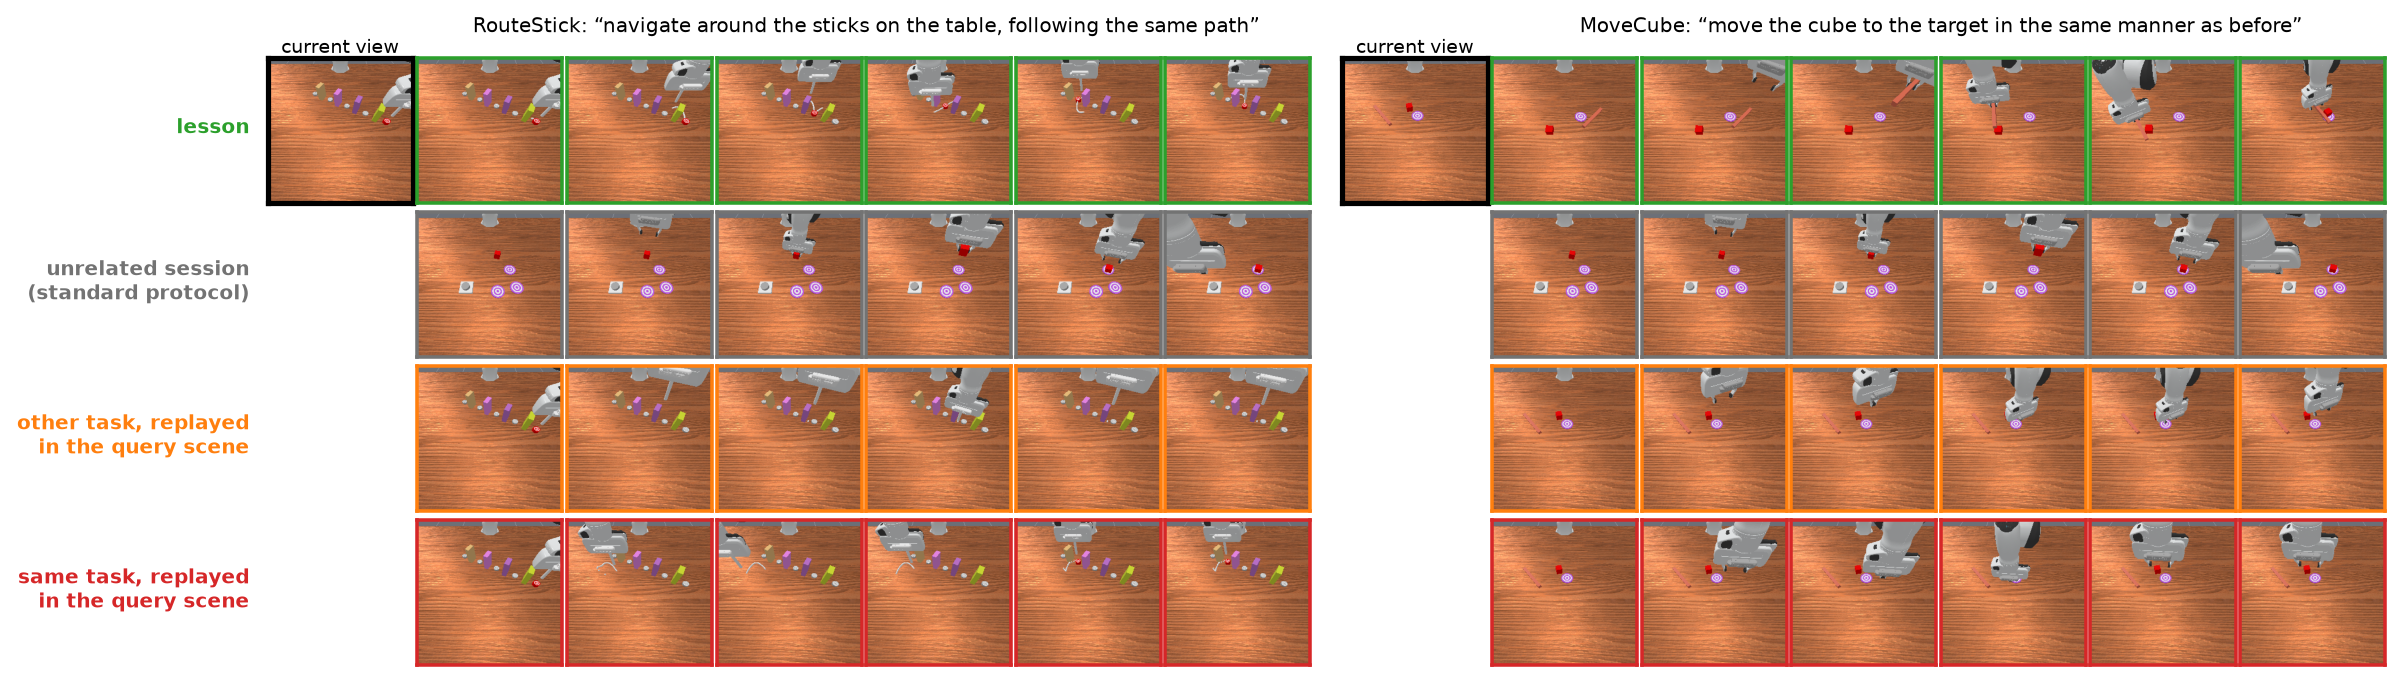
\includegraphics[width=\linewidth]{fig/qualitative.png}
\caption{Sessions of one test episode per task: six evenly spaced frames of the lesson, of an unrelated session (standard protocol), of a replay of another task recorded in the query scene (hard condition) and of a replay of the same task recorded in the query scene (same-task competitors). Black border: the view at the start of execution. Closed-loop success for the last row's condition: instruction router $.44$ (RouteStick) and $.48$ (MoveCube) against $.68$ and $.82$ with oracle routing.}
\label{fig:qual}
\end{figure}

\textbf{The manager, step by step.} Fig.~\ref{fig:algo} states the label-free manager used for the instruction-router rows.

\begin{figure}[h]
\centering\small
\fbox{\parbox{0.94\linewidth}{
\textbf{Input:} buffer frames $0..T$ with session boundaries; start $H$ of the current episode; instruction $g$; budget $B{=}32$; image and text encoders $\phi,\psi$ of a frozen SigLIP model; gate margin $\delta{=}.03$.\\[2pt]
\textbf{Once per episode (routing).}\\
\hspace*{1em}1. For each stored session $s$:\\
\hspace*{2.2em}$\mathrm{scene}_s=\max_{f\in s}\cos(\phi(f),\phi(o_H))$,\quad $\mathrm{text}_s=\max_{f\in s}\cos(\phi(f),\psi(g))$.\\
\hspace*{1em}2. Candidates $C=\{s:\mathrm{scene}_s\ge\max_{s'}\mathrm{scene}_{s'}-\delta\}$;\\
\hspace*{2.2em}$s^\star=\arg\max_{s\in C}\mathrm{text}_s$, with frames $[a,b)$ and $D=b-a$.\\[2pt]
\textbf{Every step (allocation and positions).}\\
\hspace*{1em}3. Select $B$ indices evenly over the concatenation of $[a,b)$ and $[H,T]$ (all of them if fewer than $B$).\\
\hspace*{1em}4. Re-index: a selected frame $i$ gets time position $i-a$ if $i<b$, and $D+(i-H)$ otherwise.\\
\hspace*{1em}5. Run the frozen policy on the selected frames at these positions.
}}
\caption{The label-free manager (instruction router + even comb + re-indexing). Steps 3--5 alone, with $s^\star$ given, are the lesson oracle; replacing steps 1--2 by per-step cosine similarity on the policy's own features gives retrieval + re-index.}
\label{fig:algo}
\end{figure}

\textbf{Intervals for the main tables.} Table~\ref{tab:ci} gives the paired differences behind Tables~\ref{tab:general} and~\ref{tab:hardstats} with their intervals.

\begin{table}[h]
\centering\small
\caption{Paired differences in success with Bonett--Price 95\% intervals ($n{=}50$ common episodes). ``Fix'': retrieval + re-index; ``router'': the label-free instruction router; hard-condition $k{=}0$ cells as in Table~\ref{tab:hardstats}.}
\label{tab:ci}
\setlength{\tabcolsep}{5pt}
\input{\ctrlroot ci_table}
\end{table}
 / \input{../controls}); numbers from results/robomme/paired_tests.txt.
\providecommand{\ctrlroot}{}
\section{Matched Controls}
\label{app:controls}

All cells in this section use the released FrameSamp-Modul checkpoint on the test split, $n{=}50$ episodes on the seeds, scenes and distractors of the main tables. Differences are paired, with Bonett--Price 95\% intervals and exact McNemar $p$-values.

\begin{figure}[h]
\centering
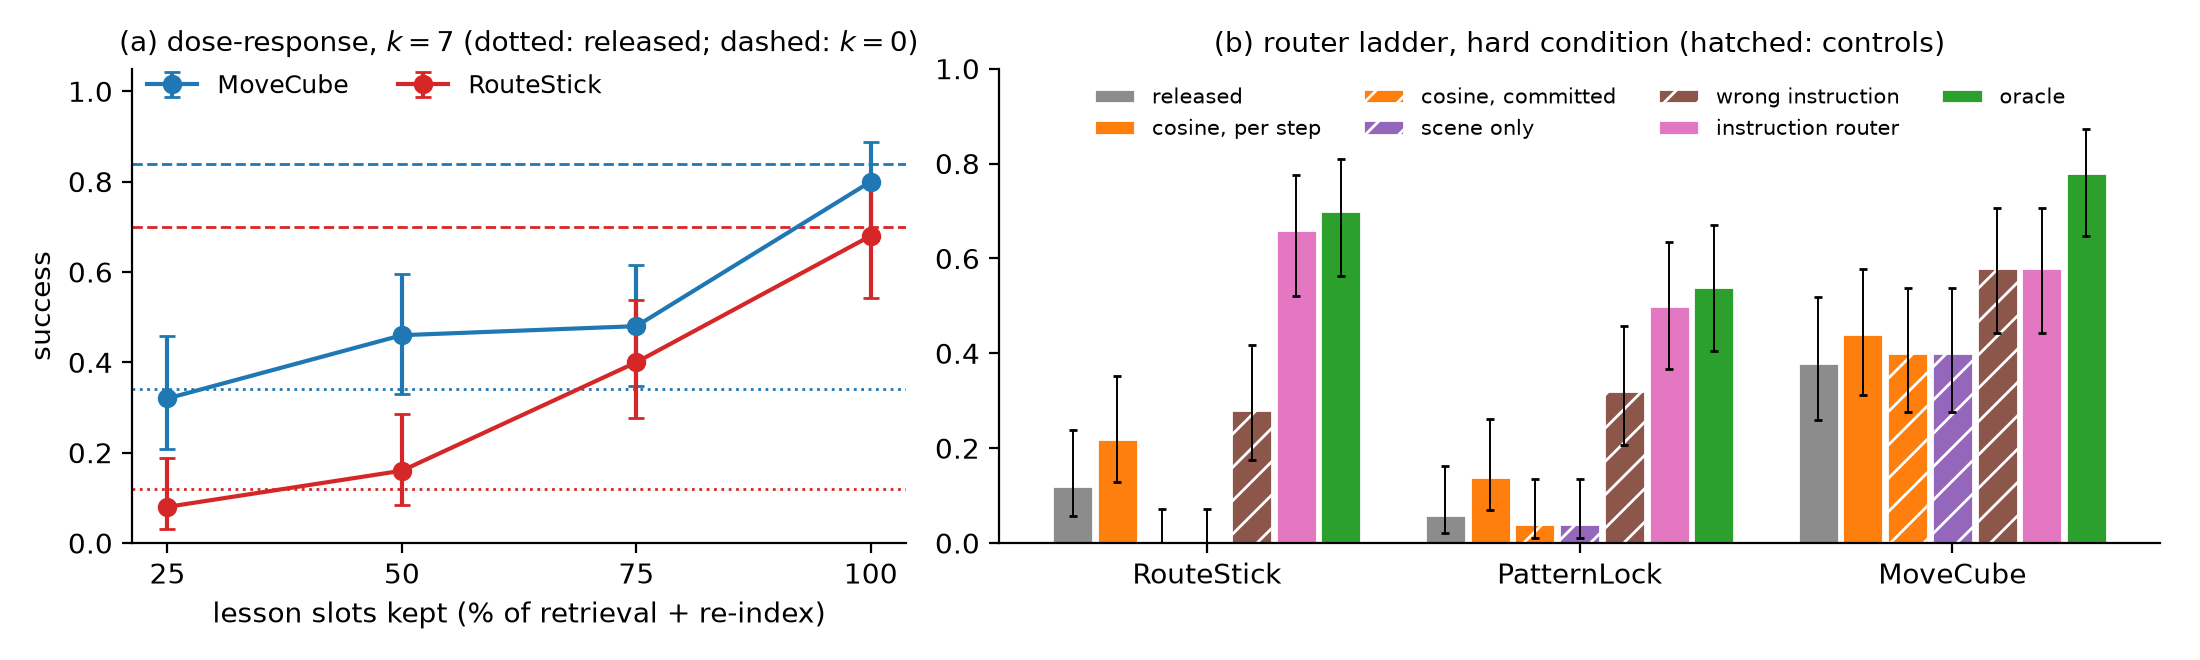
\includegraphics[width=\linewidth]{fig/controls.png}
\caption{(a)~Allocation dose-response on retrieval + re-index's own layout at $k{=}7$: success against the fraction of its lesson slots kept, the freed slots given to distractor frames (100\%: retrieval + re-index). (b)~Router ladder in the hard condition (Table~\ref{tab:ladder}). Wilson 95\% intervals, $n{=}50$ per cell.}
\label{fig:controls}
\end{figure}

\textbf{Router ladder (hard condition).} Three controls separate the parts of the instruction router. \sys{cosine, committed}: the policy-feature cosine retrieval of the main text, deciding once per episode. \sys{scene only}: the router's own encoder, gate and single decision, choosing the session most similar to the current view and never reading the instruction. \sys{wrong instruction}: the full router given the instruction of another task family, fixed per episode. Table~\ref{tab:ladder}: commitment and the encoder contribute nothing by themselves; both committed appearance routers choose a same-scene replay in every episode on all three tasks and score at or below per-step cosine retrieval (RouteStick $.22\to.00$, $p=.001$). The correct instruction is worth $+.38$ $[.22,.51]$ over the wrong one on RouteStick ($p=4\times10^{-6}$) and $+.18$ $[.02,.33]$ on PatternLock ($p=.049$). On MoveCube it is worth nothing ($.58$ vs $.58$, eight discordant episodes each way): the router's gain over the released model there does not come from reading the instruction. A wrong instruction still beats the released model on PatternLock ($+.26$, $p=.002$) and MoveCube ($+.20$, $p=.02$), because any text query breaks the appearance tie among the same-scene sessions and lands on the lesson in $.37$--$.41$ of the slots.

\begin{table}[h]
\centering\small
\caption{Router ladder, hard condition ($k{=}7$, three same-scene replays, $n{=}50$). The three middle columns are the controls; routed systems are re-indexed.}
\label{tab:ladder}
\setlength{\tabcolsep}{5pt}
\begin{tabular}{lccccccc}
\toprule
 & & cosine, & cosine, & scene & wrong & instruction & \\
task & released & per step & committed & only & instruction & router & oracle\\
\midrule
RouteStick & .12 & .22 & .00 & .00 & .28 & .66 & .70\\
PatternLock & .06 & .14 & .04 & .04 & .32 & .50 & .54\\
MoveCube & .38 & .44 & .40 & .40 & .58 & .58 & .78\\
\bottomrule
\end{tabular}
\end{table}

\textbf{Comb isolation.} At $k{=}0$ we keep the released sampler's lesson frames and their number and change only how the current-episode slots are laid out: the most recent frames densely, or every fourth frame back from the present (Table~\ref{tab:comb}). The dense window costs $.50$ $[.33,.64]$ on MoveCube ($p=4\times10^{-7}$) and $.16$ $[.02,.29]$ on VideoPlaceButton ($p=.04$), and its episodes run to the time limit; stride four is within $.10$ $[-.03,.22]$ and $.02$ $[-.09,.13]$ of the released layout. The policy needs its own episode spread over time; it does not need the exact even comb.

\begin{table}[h]
\centering\small
\caption{Left: comb isolation at $k{=}0$ (lesson frames and counts identical in all three columns). Right: index magnitude against relative gap, MoveCube at $k{=}0$ with the released frames (only positions change).}
\label{tab:comb}
\setlength{\tabcolsep}{5pt}
\begin{tabular}{lccc}
\toprule
task & released (even) & stride 4 & dense recent\\
\midrule
MoveCube & .84 & .74 & .34\\
VideoPlaceButton & .58 & .56 & .42\\
\bottomrule
\end{tabular}\qquad
\begin{tabular}{lc}
\toprule
positions & MoveCube\\
\midrule
trained layout & .84\\
current episode $+480$ & .62\\
every frame $+480$ (gap kept) & .68\\
\bottomrule
\end{tabular}
\end{table}

\textbf{Index magnitude or relative gap.} Moving only the current episode's positions 480 steps later costs $.22$ $[.07,.36]$ on MoveCube ($p=.007$). Moving \emph{every} position 480 steps later, which keeps the gap between lesson and episode at its trained value, costs $.16$ $[.03,.28]$ ($p=.02$), and the two do not differ ($+.06$ $[-.08,.19]$). The loss follows the absolute index, not the gap, which is why compacting to the trained range is the fix.

\textbf{Session boundaries.} The managers are given session boundaries. On RouteStick in the hard condition, merging the lesson with its neighbouring session leaves the instruction router unchanged ($.64$ vs $.66$, $-.02$ $[-.13,.09]$). Splitting the lesson at its midpoint is fatal ($.08$, $p=3\times10^{-8}$): the router commits to one half and the policy sees half a route. A deployed segmenter should err towards coarse sessions.

\textbf{Allocation dose-response.} At $k{=}7$ on the standard protocol we fix the number of slots given to the lesson, the current episode and the distractor sessions (Table~\ref{tab:dose}). Success rises with the lesson's slots on both tasks (8 to 24 slots: MoveCube $+.22$, $p=.013$; RouteStick $+.34$, $p=8\times10^{-5}$), and re-indexing changes no cell (all paired differences within $.06$). With eight or fewer lesson slots the policy is at its no-lesson floor. The lesson count is not sufficient, however: with 24 lesson slots, no distractor frame in memory and trained positions, both tasks remain below retrieval + re-index (MoveCube $-.28$, $p=.013$; RouteStick $-.24$, $p=.004$), whose only difference is that the current episode's share grows with the episode instead of staying at eight slots. On RouteStick an even subset of 24 lesson frames beats a random subset of 24 ($.48$ vs $.30$, $p=.004$); at 16 slots the two do not differ. A last series varies the share on a schedule that does reach the reference: retrieval + re-index's own comb over lesson and current episode, with only 25, 50 or 75\% of its lesson slots kept and the freed slots given to distractor frames (lesson share $.2$, $.4$, $.55$; reference $.87$--$.89$). Success is monotone in the fraction kept on both tasks (Fig.~\ref{fig:controls}a), MoveCube $.32/.46/.48/.80$ and RouteStick $.08/.16/.40/.68$ at $25/50/75/100\%$ ($25$ vs $100\%$: $+.48$ $[.29,.63]$, $p=8\times10^{-6}$, and $+.60$ $[.43,.72]$, $p=2\times10^{-9}$), and at 25\% it equals the released model ($-.02$, $-.04$). The curve is convex: giving up the last quarter of the lesson's slots costs $.32$ $[.13,.48]$ and $.28$ $[.12,.42]$ ($p=.002$, $.001$), about what the fixed 24-slot cells lose with no distractor frame in memory. The slot share of Fig.~\ref{fig:mechanism} is therefore causal on the trained layout and steep near the top: the policy needs close to the whole lesson comb, and a partial share buys less than its proportion.

\begin{table}[h]
\centering\small
\caption{Allocation dose-response, standard protocol, $k{=}7$: success by slots given to the lesson / current episode / distractor sessions (32 in total). Upper rows at recorded positions, lower rows re-indexed. 24r: a random instead of an even subset of 24 lesson frames. Reference: retrieval + re-index, which gives every history slot to the lesson and lets the current episode's share grow.}
\label{tab:dose}
\setlength{\tabcolsep}{3pt}
\begin{tabular}{lccccccccc|c}
\toprule
lesson/episode/distr. & 0/16/16 & 4/16/12 & 8/16/8 & 12/16/4 & 16/16/0 & 16/8/8 & 20/8/4 & 24/8/0 & 24r/8/0 & ref.\\
\midrule
MoveCube & .40 & .36 & .36 & .38 & .38 & .42 & .32 & .50 & .46 & .80\\
RouteStick & .10 & .10 & .06 & .14 & .38 & .36 & .52 & .48 & .30 & .68\\
\midrule
MoveCube, re-indexed & & & .30 & & .44 & & & .52 & & .80\\
RouteStick, re-indexed & & & .10 & & .38 & & & .44 & & .68\\
\bottomrule
\end{tabular}
\end{table}

\textbf{Same-task competitors.} The hard condition's replays are motions of other task families. In a stricter variant the three same-scene sessions replay other recorded episodes of the \emph{same} task (another cube target) in the query scene. On MoveCube: released $.32$, cosine retrieval + re-index $.42$, instruction router $.48$, lesson oracle + re-index $.82$ ($k{=}0$: $.84$; oracle against $k{=}0$ $-.02$ $[-.12,.08]$). The router is not better than cosine retrieval ($+.06$ $[-.13,.25]$) and is far below the oracle ($p=8\times10^{-5}$). Offline, scene-plus-instruction routing picks the lesson in $.46$ of MoveCube and $.64$ of RouteStick scenes (chance $.25$; scene-only $.00$): the instruction is the same for every competitor, and what remains is that the lesson is a video and the competitors are robot replays. RouteStick closed loop gives the same picture: released $.18$, cosine retrieval + re-index $.30$, instruction router $.44$, oracle $.68$ ($k{=}0$: $.70$; $-.02$ $[-.08,.05]$); the router beats the released model ($+.26$ $[.07,.43]$, $p=.011$) but not cosine retrieval ($+.14$ $[-.05,.32]$) and is below the oracle ($p=5\times10^{-4}$). Learned routers were never trained on such competitors; applied unchanged, the in-task router of \S\ref{sec:hard} transfers on MoveCube ($.74$, 41 of 50 episodes routed to the lesson; $-.08$ $[-.19,.04]$ against the oracle, $+.26$ $[.08,.42]$ over the instruction router, $p=.007$) and not on RouteStick (in-task $.34$, 26 of 50; leave-one-task-out $.20$, 12 of 50; both below the oracle, $p\le8\times10^{-5}$). Allocation still recovers the no-interference level when the lesson is found; none of our label-free routers finds it reliably among same-task sessions, and a label-trained one does so on one task of two. We note that these replays start from the reset query state, so ``the session least like the current view'' would identify the lesson in every episode; we do not use this cue, which is a property of the construction.

\textbf{What a router sees.} Fig.~\ref{fig:qual} shows the sessions of one test episode per task (episode 3 of each, chosen without reference to outcomes) as the evaluator stores them. The unrelated session of the standard protocol is in another scene, so any similarity to the current view rejects it. A replay recorded in the query scene begins at the current view itself, so cosine retrieval prefers it to the lesson. On RouteStick the lesson shows the stick tracing a path among the sticks on the table, which a single frame carries and the instruction names; a replay of another task does not, and the instruction router separates them. On MoveCube the lesson is a brief push in a sparse scene and looks much like any arm moving over the cube. A replay of the \emph{same} task shows the instructed content by construction, on both tasks, which is why no instruction-based score separates it from the lesson.

\begin{figure}[h]
\centering
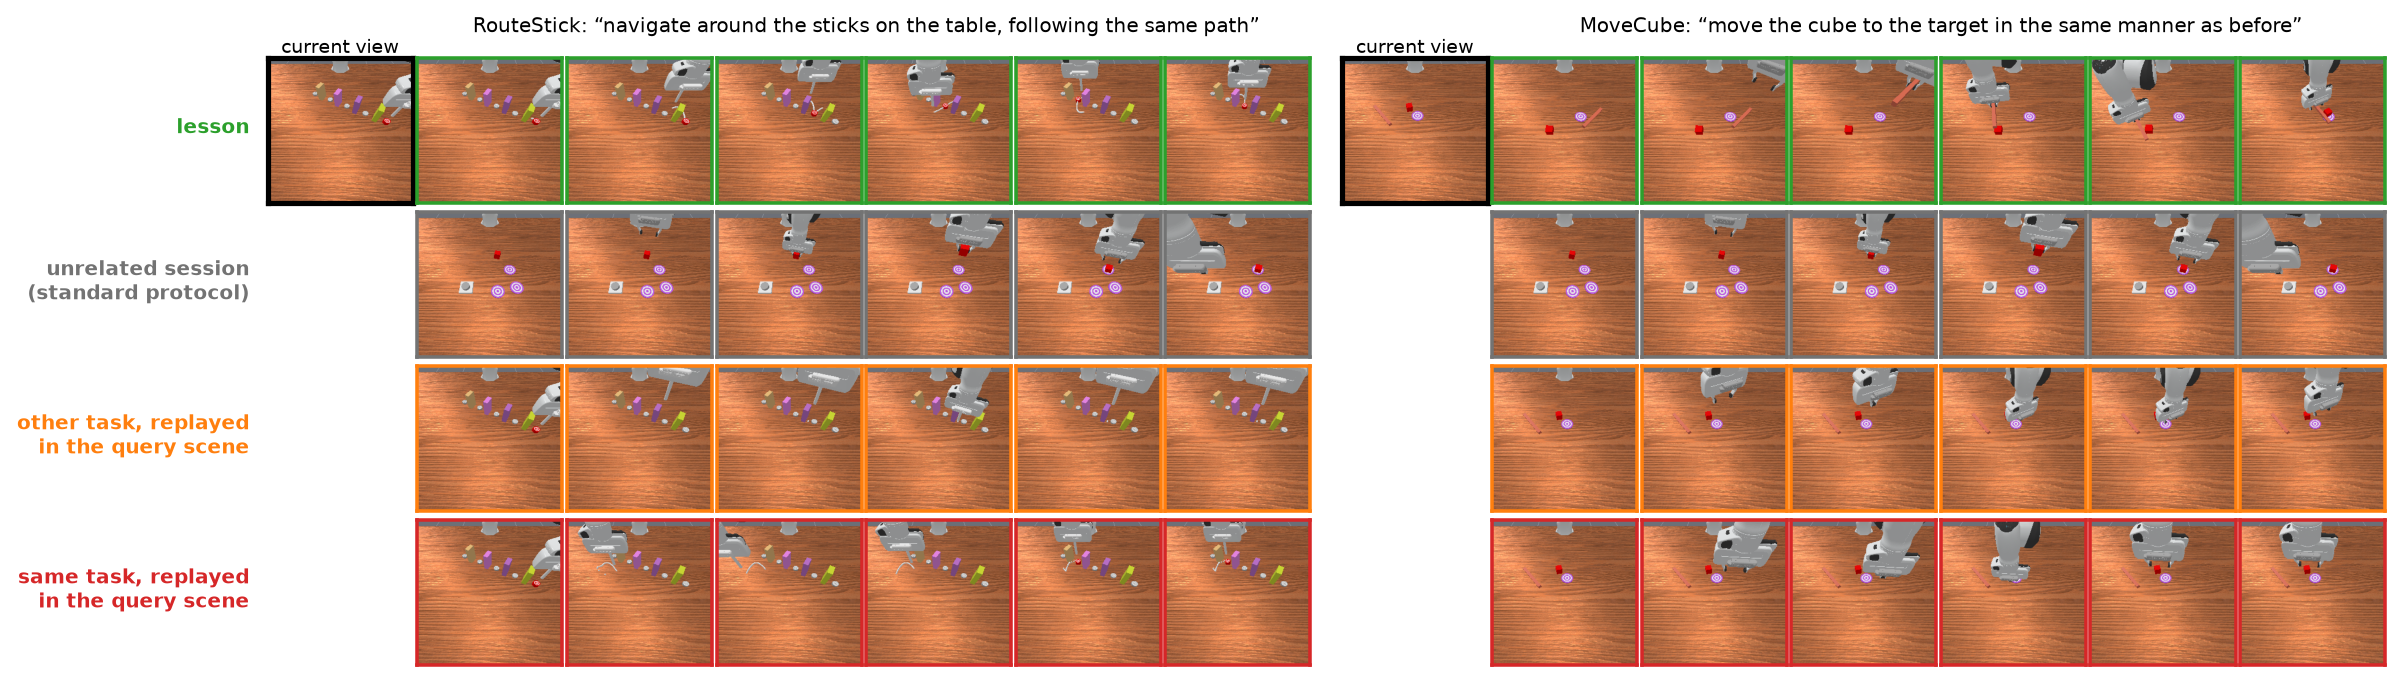
\includegraphics[width=\linewidth]{fig/qualitative.png}
\caption{Sessions of one test episode per task: six evenly spaced frames of the lesson, of an unrelated session (standard protocol), of a replay of another task recorded in the query scene (hard condition) and of a replay of the same task recorded in the query scene (same-task competitors). Black border: the view at the start of execution. Closed-loop success for the last row's condition: instruction router $.44$ (RouteStick) and $.48$ (MoveCube) against $.68$ and $.82$ with oracle routing.}
\label{fig:qual}
\end{figure}

\textbf{The manager, step by step.} Fig.~\ref{fig:algo} states the label-free manager used for the instruction-router rows.

\begin{figure}[h]
\centering\small
\fbox{\parbox{0.94\linewidth}{
\textbf{Input:} buffer frames $0..T$ with session boundaries; start $H$ of the current episode; instruction $g$; budget $B{=}32$; image and text encoders $\phi,\psi$ of a frozen SigLIP model; gate margin $\delta{=}.03$.\\[2pt]
\textbf{Once per episode (routing).}\\
\hspace*{1em}1. For each stored session $s$:\\
\hspace*{2.2em}$\mathrm{scene}_s=\max_{f\in s}\cos(\phi(f),\phi(o_H))$,\quad $\mathrm{text}_s=\max_{f\in s}\cos(\phi(f),\psi(g))$.\\
\hspace*{1em}2. Candidates $C=\{s:\mathrm{scene}_s\ge\max_{s'}\mathrm{scene}_{s'}-\delta\}$;\\
\hspace*{2.2em}$s^\star=\arg\max_{s\in C}\mathrm{text}_s$, with frames $[a,b)$ and $D=b-a$.\\[2pt]
\textbf{Every step (allocation and positions).}\\
\hspace*{1em}3. Select $B$ indices evenly over the concatenation of $[a,b)$ and $[H,T]$ (all of them if fewer than $B$).\\
\hspace*{1em}4. Re-index: a selected frame $i$ gets time position $i-a$ if $i<b$, and $D+(i-H)$ otherwise.\\
\hspace*{1em}5. Run the frozen policy on the selected frames at these positions.
}}
\caption{The label-free manager (instruction router + even comb + re-indexing). Steps 3--5 alone, with $s^\star$ given, are the lesson oracle; replacing steps 1--2 by per-step cosine similarity on the policy's own features gives retrieval + re-index.}
\label{fig:algo}
\end{figure}

\textbf{Intervals for the main tables.} Table~\ref{tab:ci} gives the paired differences behind Tables~\ref{tab:general} and~\ref{tab:hardstats} with their intervals.

\begin{table}[h]
\centering\small
\caption{Paired differences in success with Bonett--Price 95\% intervals ($n{=}50$ common episodes). ``Fix'': retrieval + re-index; ``router'': the label-free instruction router; hard-condition $k{=}0$ cells as in Table~\ref{tab:hardstats}.}
\label{tab:ci}
\setlength{\tabcolsep}{5pt}
\input{\ctrlroot ci_table}
\end{table}
 / \input{../controls}); numbers from results/robomme/paired_tests.txt.
\providecommand{\ctrlroot}{}
\section{Matched Controls}
\label{app:controls}

All cells in this section use the released FrameSamp-Modul checkpoint on the test split, $n{=}50$ episodes on the seeds, scenes and distractors of the main tables. Differences are paired, with Bonett--Price 95\% intervals and exact McNemar $p$-values.

\begin{figure}[h]
\centering
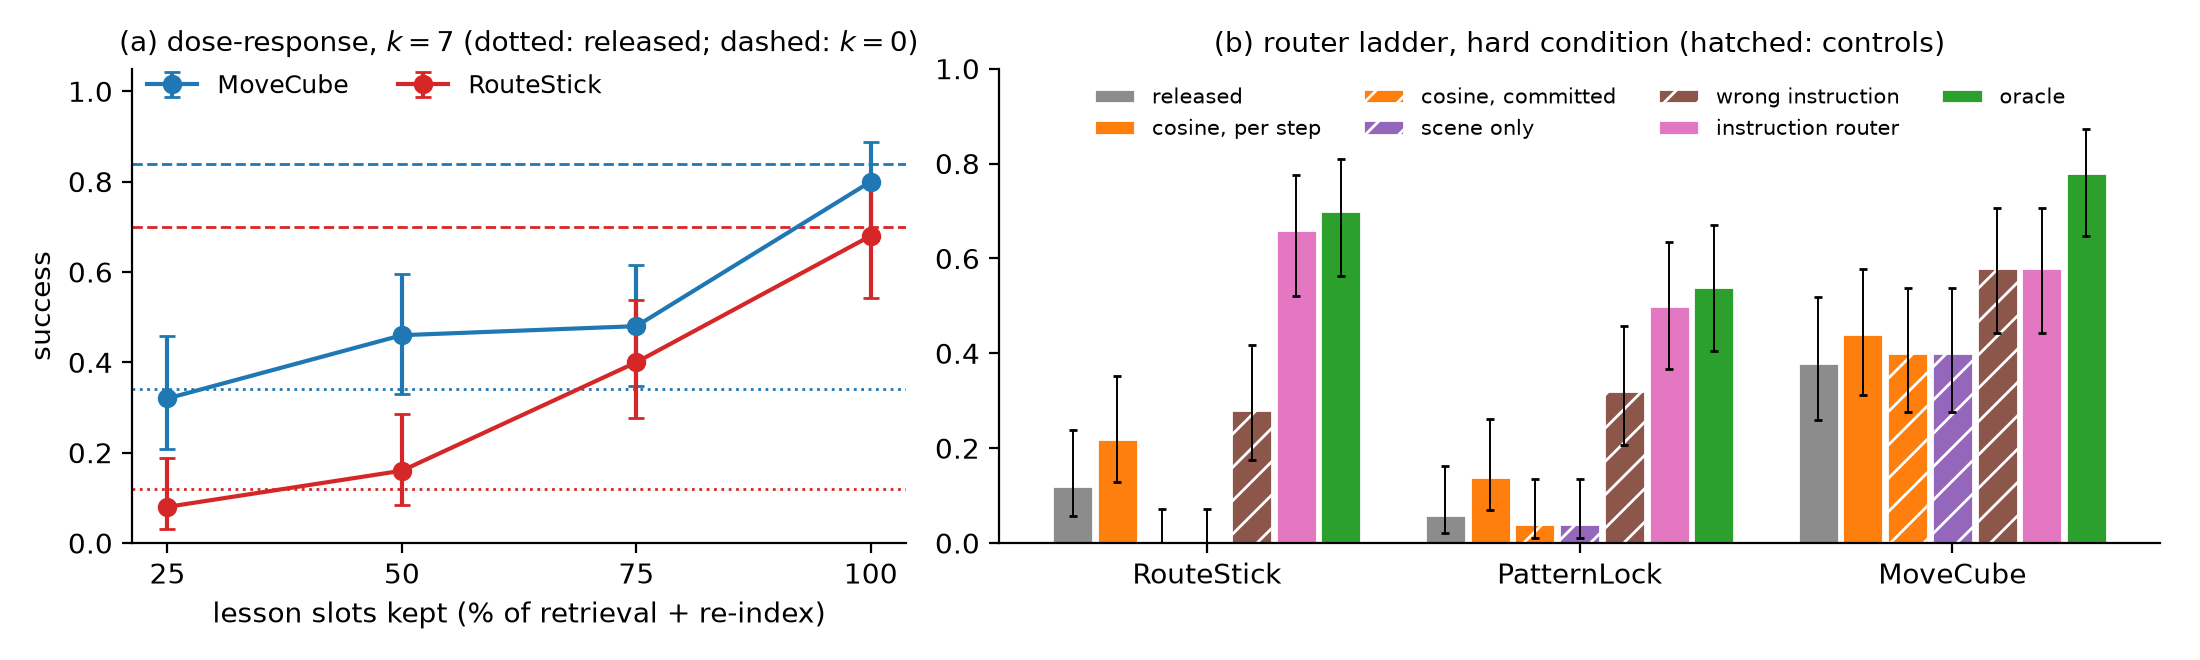
\includegraphics[width=\linewidth]{fig/controls.png}
\caption{(a)~Allocation dose-response on retrieval + re-index's own layout at $k{=}7$: success against the fraction of its lesson slots kept, the freed slots given to distractor frames (100\%: retrieval + re-index). (b)~Router ladder in the hard condition (Table~\ref{tab:ladder}). Wilson 95\% intervals, $n{=}50$ per cell.}
\label{fig:controls}
\end{figure}

\textbf{Router ladder (hard condition).} Three controls separate the parts of the instruction router. \sys{cosine, committed}: the policy-feature cosine retrieval of the main text, deciding once per episode. \sys{scene only}: the router's own encoder, gate and single decision, choosing the session most similar to the current view and never reading the instruction. \sys{wrong instruction}: the full router given the instruction of another task family, fixed per episode. Table~\ref{tab:ladder}: commitment and the encoder contribute nothing by themselves; both committed appearance routers choose a same-scene replay in every episode on all three tasks and score at or below per-step cosine retrieval (RouteStick $.22\to.00$, $p=.001$). The correct instruction is worth $+.38$ $[.22,.51]$ over the wrong one on RouteStick ($p=4\times10^{-6}$) and $+.18$ $[.02,.33]$ on PatternLock ($p=.049$). On MoveCube it is worth nothing ($.58$ vs $.58$, eight discordant episodes each way): the router's gain over the released model there does not come from reading the instruction. A wrong instruction still beats the released model on PatternLock ($+.26$, $p=.002$) and MoveCube ($+.20$, $p=.02$), because any text query breaks the appearance tie among the same-scene sessions and lands on the lesson in $.37$--$.41$ of the slots.

\begin{table}[h]
\centering\small
\caption{Router ladder, hard condition ($k{=}7$, three same-scene replays, $n{=}50$). The three middle columns are the controls; routed systems are re-indexed.}
\label{tab:ladder}
\setlength{\tabcolsep}{5pt}
\begin{tabular}{lccccccc}
\toprule
 & & cosine, & cosine, & scene & wrong & instruction & \\
task & released & per step & committed & only & instruction & router & oracle\\
\midrule
RouteStick & .12 & .22 & .00 & .00 & .28 & .66 & .70\\
PatternLock & .06 & .14 & .04 & .04 & .32 & .50 & .54\\
MoveCube & .38 & .44 & .40 & .40 & .58 & .58 & .78\\
\bottomrule
\end{tabular}
\end{table}

\textbf{Comb isolation.} At $k{=}0$ we keep the released sampler's lesson frames and their number and change only how the current-episode slots are laid out: the most recent frames densely, or every fourth frame back from the present (Table~\ref{tab:comb}). The dense window costs $.50$ $[.33,.64]$ on MoveCube ($p=4\times10^{-7}$) and $.16$ $[.02,.29]$ on VideoPlaceButton ($p=.04$), and its episodes run to the time limit; stride four is within $.10$ $[-.03,.22]$ and $.02$ $[-.09,.13]$ of the released layout. The policy needs its own episode spread over time; it does not need the exact even comb.

\begin{table}[h]
\centering\small
\caption{Left: comb isolation at $k{=}0$ (lesson frames and counts identical in all three columns). Right: index magnitude against relative gap, MoveCube at $k{=}0$ with the released frames (only positions change).}
\label{tab:comb}
\setlength{\tabcolsep}{5pt}
\begin{tabular}{lccc}
\toprule
task & released (even) & stride 4 & dense recent\\
\midrule
MoveCube & .84 & .74 & .34\\
VideoPlaceButton & .58 & .56 & .42\\
\bottomrule
\end{tabular}\qquad
\begin{tabular}{lc}
\toprule
positions & MoveCube\\
\midrule
trained layout & .84\\
current episode $+480$ & .62\\
every frame $+480$ (gap kept) & .68\\
\bottomrule
\end{tabular}
\end{table}

\textbf{Index magnitude or relative gap.} Moving only the current episode's positions 480 steps later costs $.22$ $[.07,.36]$ on MoveCube ($p=.007$). Moving \emph{every} position 480 steps later, which keeps the gap between lesson and episode at its trained value, costs $.16$ $[.03,.28]$ ($p=.02$), and the two do not differ ($+.06$ $[-.08,.19]$). The loss follows the absolute index, not the gap, which is why compacting to the trained range is the fix.

\textbf{Session boundaries.} The managers are given session boundaries. On RouteStick in the hard condition, merging the lesson with its neighbouring session leaves the instruction router unchanged ($.64$ vs $.66$, $-.02$ $[-.13,.09]$). Splitting the lesson at its midpoint is fatal ($.08$, $p=3\times10^{-8}$): the router commits to one half and the policy sees half a route. A deployed segmenter should err towards coarse sessions.

\textbf{Allocation dose-response.} At $k{=}7$ on the standard protocol we fix the number of slots given to the lesson, the current episode and the distractor sessions (Table~\ref{tab:dose}). Success rises with the lesson's slots on both tasks (8 to 24 slots: MoveCube $+.22$, $p=.013$; RouteStick $+.34$, $p=8\times10^{-5}$), and re-indexing changes no cell (all paired differences within $.06$). With eight or fewer lesson slots the policy is at its no-lesson floor. The lesson count is not sufficient, however: with 24 lesson slots, no distractor frame in memory and trained positions, both tasks remain below retrieval + re-index (MoveCube $-.28$, $p=.013$; RouteStick $-.24$, $p=.004$), whose only difference is that the current episode's share grows with the episode instead of staying at eight slots. On RouteStick an even subset of 24 lesson frames beats a random subset of 24 ($.48$ vs $.30$, $p=.004$); at 16 slots the two do not differ. A last series varies the share on a schedule that does reach the reference: retrieval + re-index's own comb over lesson and current episode, with only 25, 50 or 75\% of its lesson slots kept and the freed slots given to distractor frames (lesson share $.2$, $.4$, $.55$; reference $.87$--$.89$). Success is monotone in the fraction kept on both tasks (Fig.~\ref{fig:controls}a), MoveCube $.32/.46/.48/.80$ and RouteStick $.08/.16/.40/.68$ at $25/50/75/100\%$ ($25$ vs $100\%$: $+.48$ $[.29,.63]$, $p=8\times10^{-6}$, and $+.60$ $[.43,.72]$, $p=2\times10^{-9}$), and at 25\% it equals the released model ($-.02$, $-.04$). The curve is convex: giving up the last quarter of the lesson's slots costs $.32$ $[.13,.48]$ and $.28$ $[.12,.42]$ ($p=.002$, $.001$), about what the fixed 24-slot cells lose with no distractor frame in memory. The slot share of Fig.~\ref{fig:mechanism} is therefore causal on the trained layout and steep near the top: the policy needs close to the whole lesson comb, and a partial share buys less than its proportion.

\begin{table}[h]
\centering\small
\caption{Allocation dose-response, standard protocol, $k{=}7$: success by slots given to the lesson / current episode / distractor sessions (32 in total). Upper rows at recorded positions, lower rows re-indexed. 24r: a random instead of an even subset of 24 lesson frames. Reference: retrieval + re-index, which gives every history slot to the lesson and lets the current episode's share grow.}
\label{tab:dose}
\setlength{\tabcolsep}{3pt}
\begin{tabular}{lccccccccc|c}
\toprule
lesson/episode/distr. & 0/16/16 & 4/16/12 & 8/16/8 & 12/16/4 & 16/16/0 & 16/8/8 & 20/8/4 & 24/8/0 & 24r/8/0 & ref.\\
\midrule
MoveCube & .40 & .36 & .36 & .38 & .38 & .42 & .32 & .50 & .46 & .80\\
RouteStick & .10 & .10 & .06 & .14 & .38 & .36 & .52 & .48 & .30 & .68\\
\midrule
MoveCube, re-indexed & & & .30 & & .44 & & & .52 & & .80\\
RouteStick, re-indexed & & & .10 & & .38 & & & .44 & & .68\\
\bottomrule
\end{tabular}
\end{table}

\textbf{Same-task competitors.} The hard condition's replays are motions of other task families. In a stricter variant the three same-scene sessions replay other recorded episodes of the \emph{same} task (another cube target) in the query scene. On MoveCube: released $.32$, cosine retrieval + re-index $.42$, instruction router $.48$, lesson oracle + re-index $.82$ ($k{=}0$: $.84$; oracle against $k{=}0$ $-.02$ $[-.12,.08]$). The router is not better than cosine retrieval ($+.06$ $[-.13,.25]$) and is far below the oracle ($p=8\times10^{-5}$). Offline, scene-plus-instruction routing picks the lesson in $.46$ of MoveCube and $.64$ of RouteStick scenes (chance $.25$; scene-only $.00$): the instruction is the same for every competitor, and what remains is that the lesson is a video and the competitors are robot replays. RouteStick closed loop gives the same picture: released $.18$, cosine retrieval + re-index $.30$, instruction router $.44$, oracle $.68$ ($k{=}0$: $.70$; $-.02$ $[-.08,.05]$); the router beats the released model ($+.26$ $[.07,.43]$, $p=.011$) but not cosine retrieval ($+.14$ $[-.05,.32]$) and is below the oracle ($p=5\times10^{-4}$). Learned routers were never trained on such competitors; applied unchanged, the in-task router of \S\ref{sec:hard} transfers on MoveCube ($.74$, 41 of 50 episodes routed to the lesson; $-.08$ $[-.19,.04]$ against the oracle, $+.26$ $[.08,.42]$ over the instruction router, $p=.007$) and not on RouteStick (in-task $.34$, 26 of 50; leave-one-task-out $.20$, 12 of 50; both below the oracle, $p\le8\times10^{-5}$). Allocation still recovers the no-interference level when the lesson is found; none of our label-free routers finds it reliably among same-task sessions, and a label-trained one does so on one task of two. We note that these replays start from the reset query state, so ``the session least like the current view'' would identify the lesson in every episode; we do not use this cue, which is a property of the construction.

\textbf{What a router sees.} Fig.~\ref{fig:qual} shows the sessions of one test episode per task (episode 3 of each, chosen without reference to outcomes) as the evaluator stores them. The unrelated session of the standard protocol is in another scene, so any similarity to the current view rejects it. A replay recorded in the query scene begins at the current view itself, so cosine retrieval prefers it to the lesson. On RouteStick the lesson shows the stick tracing a path among the sticks on the table, which a single frame carries and the instruction names; a replay of another task does not, and the instruction router separates them. On MoveCube the lesson is a brief push in a sparse scene and looks much like any arm moving over the cube. A replay of the \emph{same} task shows the instructed content by construction, on both tasks, which is why no instruction-based score separates it from the lesson.

\begin{figure}[h]
\centering
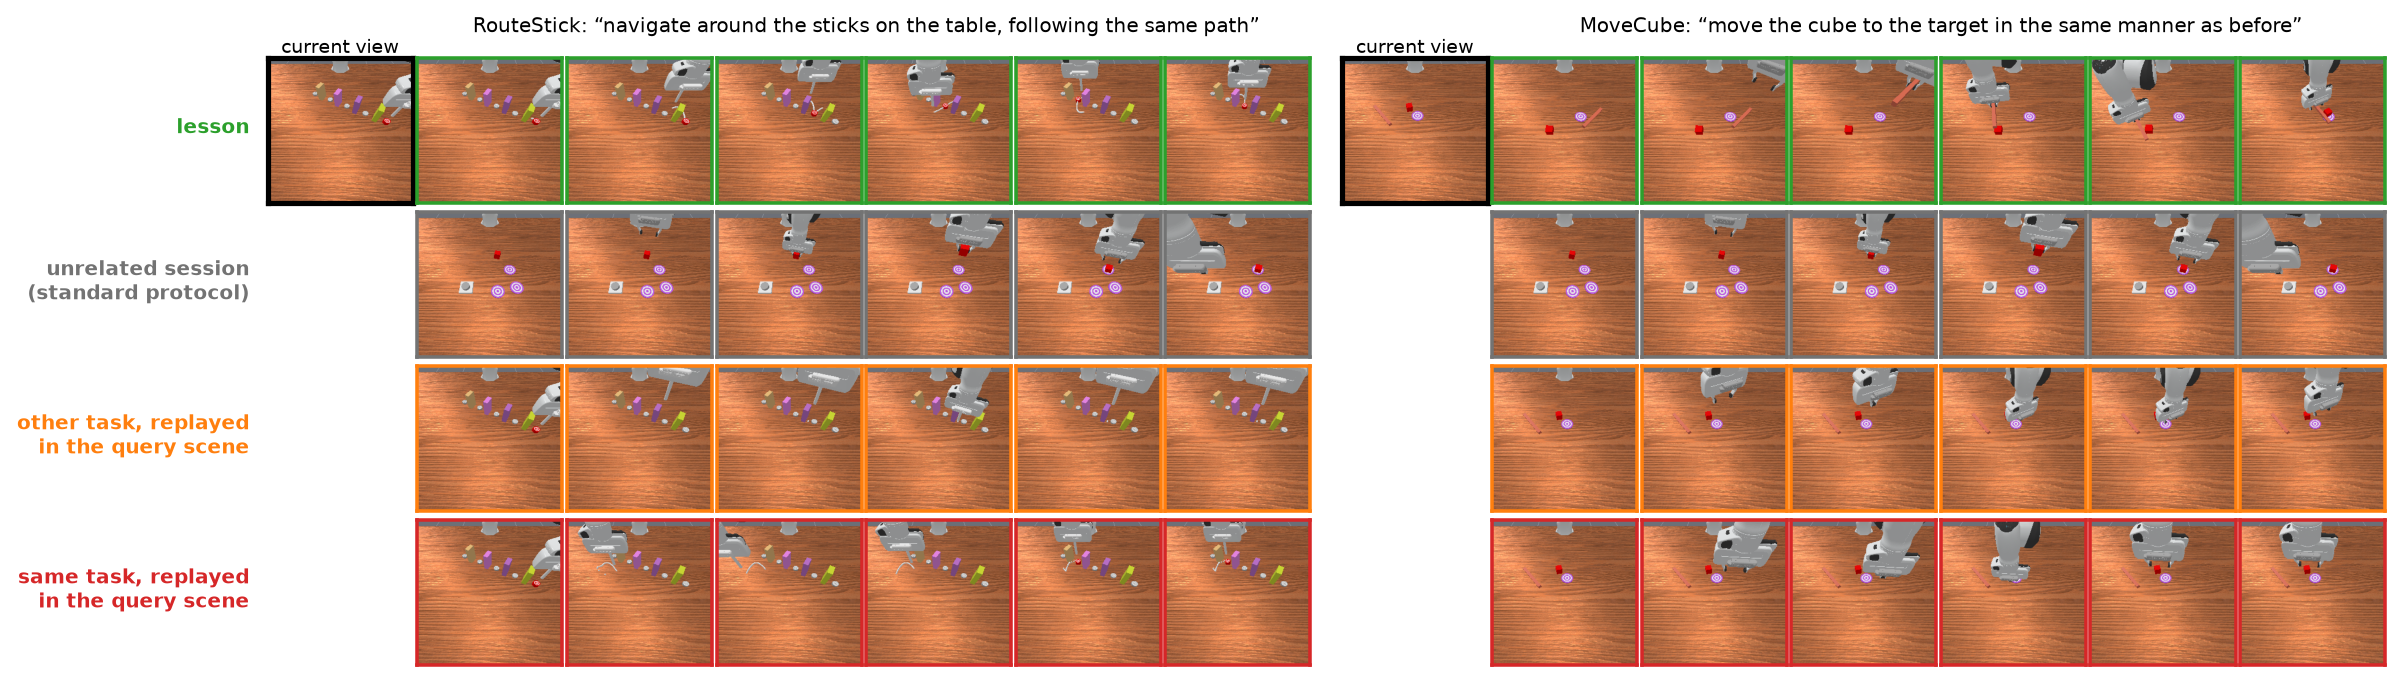
\includegraphics[width=\linewidth]{fig/qualitative.png}
\caption{Sessions of one test episode per task: six evenly spaced frames of the lesson, of an unrelated session (standard protocol), of a replay of another task recorded in the query scene (hard condition) and of a replay of the same task recorded in the query scene (same-task competitors). Black border: the view at the start of execution. Closed-loop success for the last row's condition: instruction router $.44$ (RouteStick) and $.48$ (MoveCube) against $.68$ and $.82$ with oracle routing.}
\label{fig:qual}
\end{figure}

\textbf{The manager, step by step.} Fig.~\ref{fig:algo} states the label-free manager used for the instruction-router rows.

\begin{figure}[h]
\centering\small
\fbox{\parbox{0.94\linewidth}{
\textbf{Input:} buffer frames $0..T$ with session boundaries; start $H$ of the current episode; instruction $g$; budget $B{=}32$; image and text encoders $\phi,\psi$ of a frozen SigLIP model; gate margin $\delta{=}.03$.\\[2pt]
\textbf{Once per episode (routing).}\\
\hspace*{1em}1. For each stored session $s$:\\
\hspace*{2.2em}$\mathrm{scene}_s=\max_{f\in s}\cos(\phi(f),\phi(o_H))$,\quad $\mathrm{text}_s=\max_{f\in s}\cos(\phi(f),\psi(g))$.\\
\hspace*{1em}2. Candidates $C=\{s:\mathrm{scene}_s\ge\max_{s'}\mathrm{scene}_{s'}-\delta\}$;\\
\hspace*{2.2em}$s^\star=\arg\max_{s\in C}\mathrm{text}_s$, with frames $[a,b)$ and $D=b-a$.\\[2pt]
\textbf{Every step (allocation and positions).}\\
\hspace*{1em}3. Select $B$ indices evenly over the concatenation of $[a,b)$ and $[H,T]$ (all of them if fewer than $B$).\\
\hspace*{1em}4. Re-index: a selected frame $i$ gets time position $i-a$ if $i<b$, and $D+(i-H)$ otherwise.\\
\hspace*{1em}5. Run the frozen policy on the selected frames at these positions.
}}
\caption{The label-free manager (instruction router + even comb + re-indexing). Steps 3--5 alone, with $s^\star$ given, are the lesson oracle; replacing steps 1--2 by per-step cosine similarity on the policy's own features gives retrieval + re-index.}
\label{fig:algo}
\end{figure}

\textbf{Intervals for the main tables.} Table~\ref{tab:ci} gives the paired differences behind Tables~\ref{tab:general} and~\ref{tab:hardstats} with their intervals.

\begin{table}[h]
\centering\small
\caption{Paired differences in success with Bonett--Price 95\% intervals ($n{=}50$ common episodes). ``Fix'': retrieval + re-index; ``router'': the label-free instruction router; hard-condition $k{=}0$ cells as in Table~\ref{tab:hardstats}.}
\label{tab:ci}
\setlength{\tabcolsep}{5pt}
\input{\ctrlroot ci_table}
\end{table}
 / \input{../controls}); numbers from results/robomme/paired_tests.txt.
\providecommand{\ctrlroot}{}
\section{Matched Controls}
\label{app:controls}

All cells in this section use the released FrameSamp-Modul checkpoint on the test split, $n{=}50$ episodes on the seeds, scenes and distractors of the main tables. Differences are paired, with Bonett--Price 95\% intervals and exact McNemar $p$-values.

\begin{figure}[h]
\centering
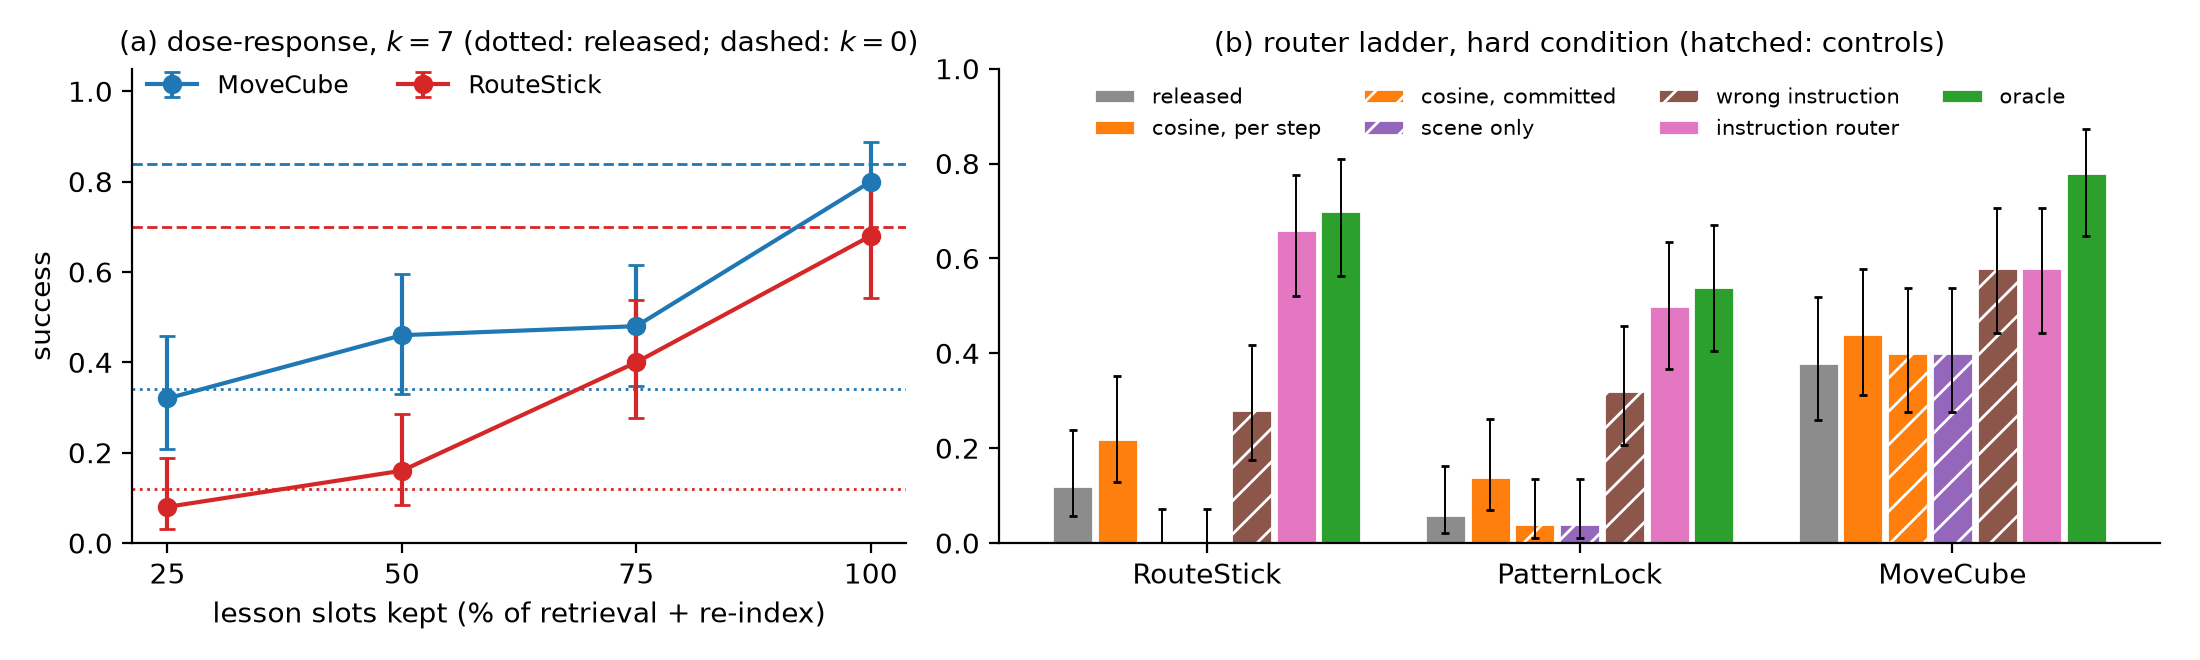
\includegraphics[width=\linewidth]{fig/controls.png}
\caption{(a)~Allocation dose-response on retrieval + re-index's own layout at $k{=}7$: success against the fraction of its lesson slots kept, the freed slots given to distractor frames (100\%: retrieval + re-index). (b)~Router ladder in the hard condition (Table~\ref{tab:ladder}). Wilson 95\% intervals, $n{=}50$ per cell.}
\label{fig:controls}
\end{figure}

\textbf{Router ladder (hard condition).} Three controls separate the parts of the instruction router. \sys{cosine, committed}: the policy-feature cosine retrieval of the main text, deciding once per episode. \sys{scene only}: the router's own encoder, gate and single decision, choosing the session most similar to the current view and never reading the instruction. \sys{wrong instruction}: the full router given the instruction of another task family, fixed per episode. Table~\ref{tab:ladder}: commitment and the encoder contribute nothing by themselves; both committed appearance routers choose a same-scene replay in every episode on all three tasks and score at or below per-step cosine retrieval (RouteStick $.22\to.00$, $p=.001$). The correct instruction is worth $+.38$ $[.22,.51]$ over the wrong one on RouteStick ($p=4\times10^{-6}$) and $+.18$ $[.02,.33]$ on PatternLock ($p=.049$). On MoveCube it is worth nothing ($.58$ vs $.58$, eight discordant episodes each way): the router's gain over the released model there does not come from reading the instruction. A wrong instruction still beats the released model on PatternLock ($+.26$, $p=.002$) and MoveCube ($+.20$, $p=.02$), because any text query breaks the appearance tie among the same-scene sessions and lands on the lesson in $.37$--$.41$ of the slots.

\begin{table}[h]
\centering\small
\caption{Router ladder, hard condition ($k{=}7$, three same-scene replays, $n{=}50$). The three middle columns are the controls; routed systems are re-indexed.}
\label{tab:ladder}
\setlength{\tabcolsep}{5pt}
\begin{tabular}{lccccccc}
\toprule
 & & cosine, & cosine, & scene & wrong & instruction & \\
task & released & per step & committed & only & instruction & router & oracle\\
\midrule
RouteStick & .12 & .22 & .00 & .00 & .28 & .66 & .70\\
PatternLock & .06 & .14 & .04 & .04 & .32 & .50 & .54\\
MoveCube & .38 & .44 & .40 & .40 & .58 & .58 & .78\\
\bottomrule
\end{tabular}
\end{table}

\textbf{Comb isolation.} At $k{=}0$ we keep the released sampler's lesson frames and their number and change only how the current-episode slots are laid out: the most recent frames densely, or every fourth frame back from the present (Table~\ref{tab:comb}). The dense window costs $.50$ $[.33,.64]$ on MoveCube ($p=4\times10^{-7}$) and $.16$ $[.02,.29]$ on VideoPlaceButton ($p=.04$), and its episodes run to the time limit; stride four is within $.10$ $[-.03,.22]$ and $.02$ $[-.09,.13]$ of the released layout. The policy needs its own episode spread over time; it does not need the exact even comb.

\begin{table}[h]
\centering\small
\caption{Left: comb isolation at $k{=}0$ (lesson frames and counts identical in all three columns). Right: index magnitude against relative gap, MoveCube at $k{=}0$ with the released frames (only positions change).}
\label{tab:comb}
\setlength{\tabcolsep}{5pt}
\begin{tabular}{lccc}
\toprule
task & released (even) & stride 4 & dense recent\\
\midrule
MoveCube & .84 & .74 & .34\\
VideoPlaceButton & .58 & .56 & .42\\
\bottomrule
\end{tabular}\qquad
\begin{tabular}{lc}
\toprule
positions & MoveCube\\
\midrule
trained layout & .84\\
current episode $+480$ & .62\\
every frame $+480$ (gap kept) & .68\\
\bottomrule
\end{tabular}
\end{table}

\textbf{Index magnitude or relative gap.} Moving only the current episode's positions 480 steps later costs $.22$ $[.07,.36]$ on MoveCube ($p=.007$). Moving \emph{every} position 480 steps later, which keeps the gap between lesson and episode at its trained value, costs $.16$ $[.03,.28]$ ($p=.02$), and the two do not differ ($+.06$ $[-.08,.19]$). The loss follows the absolute index, not the gap, which is why compacting to the trained range is the fix.

\textbf{Session boundaries.} The managers are given session boundaries. On RouteStick in the hard condition, merging the lesson with its neighbouring session leaves the instruction router unchanged ($.64$ vs $.66$, $-.02$ $[-.13,.09]$). Splitting the lesson at its midpoint is fatal ($.08$, $p=3\times10^{-8}$): the router commits to one half and the policy sees half a route. A deployed segmenter should err towards coarse sessions.

\textbf{Allocation dose-response.} At $k{=}7$ on the standard protocol we fix the number of slots given to the lesson, the current episode and the distractor sessions (Table~\ref{tab:dose}). Success rises with the lesson's slots on both tasks (8 to 24 slots: MoveCube $+.22$, $p=.013$; RouteStick $+.34$, $p=8\times10^{-5}$), and re-indexing changes no cell (all paired differences within $.06$). With eight or fewer lesson slots the policy is at its no-lesson floor. The lesson count is not sufficient, however: with 24 lesson slots, no distractor frame in memory and trained positions, both tasks remain below retrieval + re-index (MoveCube $-.28$, $p=.013$; RouteStick $-.24$, $p=.004$), whose only difference is that the current episode's share grows with the episode instead of staying at eight slots. On RouteStick an even subset of 24 lesson frames beats a random subset of 24 ($.48$ vs $.30$, $p=.004$); at 16 slots the two do not differ. A last series varies the share on a schedule that does reach the reference: retrieval + re-index's own comb over lesson and current episode, with only 25, 50 or 75\% of its lesson slots kept and the freed slots given to distractor frames (lesson share $.2$, $.4$, $.55$; reference $.87$--$.89$). Success is monotone in the fraction kept on both tasks (Fig.~\ref{fig:controls}a), MoveCube $.32/.46/.48/.80$ and RouteStick $.08/.16/.40/.68$ at $25/50/75/100\%$ ($25$ vs $100\%$: $+.48$ $[.29,.63]$, $p=8\times10^{-6}$, and $+.60$ $[.43,.72]$, $p=2\times10^{-9}$), and at 25\% it equals the released model ($-.02$, $-.04$). The curve is convex: giving up the last quarter of the lesson's slots costs $.32$ $[.13,.48]$ and $.28$ $[.12,.42]$ ($p=.002$, $.001$), about what the fixed 24-slot cells lose with no distractor frame in memory. The slot share of Fig.~\ref{fig:mechanism} is therefore causal on the trained layout and steep near the top: the policy needs close to the whole lesson comb, and a partial share buys less than its proportion.

\begin{table}[h]
\centering\small
\caption{Allocation dose-response, standard protocol, $k{=}7$: success by slots given to the lesson / current episode / distractor sessions (32 in total). Upper rows at recorded positions, lower rows re-indexed. 24r: a random instead of an even subset of 24 lesson frames. Reference: retrieval + re-index, which gives every history slot to the lesson and lets the current episode's share grow.}
\label{tab:dose}
\setlength{\tabcolsep}{3pt}
\begin{tabular}{lccccccccc|c}
\toprule
lesson/episode/distr. & 0/16/16 & 4/16/12 & 8/16/8 & 12/16/4 & 16/16/0 & 16/8/8 & 20/8/4 & 24/8/0 & 24r/8/0 & ref.\\
\midrule
MoveCube & .40 & .36 & .36 & .38 & .38 & .42 & .32 & .50 & .46 & .80\\
RouteStick & .10 & .10 & .06 & .14 & .38 & .36 & .52 & .48 & .30 & .68\\
\midrule
MoveCube, re-indexed & & & .30 & & .44 & & & .52 & & .80\\
RouteStick, re-indexed & & & .10 & & .38 & & & .44 & & .68\\
\bottomrule
\end{tabular}
\end{table}

\textbf{Same-task competitors.} The hard condition's replays are motions of other task families. In a stricter variant the three same-scene sessions replay other recorded episodes of the \emph{same} task (another cube target) in the query scene. On MoveCube: released $.32$, cosine retrieval + re-index $.42$, instruction router $.48$, lesson oracle + re-index $.82$ ($k{=}0$: $.84$; oracle against $k{=}0$ $-.02$ $[-.12,.08]$). The router is not better than cosine retrieval ($+.06$ $[-.13,.25]$) and is far below the oracle ($p=8\times10^{-5}$). Offline, scene-plus-instruction routing picks the lesson in $.46$ of MoveCube and $.64$ of RouteStick scenes (chance $.25$; scene-only $.00$): the instruction is the same for every competitor, and what remains is that the lesson is a video and the competitors are robot replays. RouteStick closed loop gives the same picture: released $.18$, cosine retrieval + re-index $.30$, instruction router $.44$, oracle $.68$ ($k{=}0$: $.70$; $-.02$ $[-.08,.05]$); the router beats the released model ($+.26$ $[.07,.43]$, $p=.011$) but not cosine retrieval ($+.14$ $[-.05,.32]$) and is below the oracle ($p=5\times10^{-4}$). Learned routers were never trained on such competitors; applied unchanged, the in-task router of \S\ref{sec:hard} transfers on MoveCube ($.74$, 41 of 50 episodes routed to the lesson; $-.08$ $[-.19,.04]$ against the oracle, $+.26$ $[.08,.42]$ over the instruction router, $p=.007$) and not on RouteStick (in-task $.34$, 26 of 50; leave-one-task-out $.20$, 12 of 50; both below the oracle, $p\le8\times10^{-5}$). Allocation still recovers the no-interference level when the lesson is found; none of our label-free routers finds it reliably among same-task sessions, and a label-trained one does so on one task of two. We note that these replays start from the reset query state, so ``the session least like the current view'' would identify the lesson in every episode; we do not use this cue, which is a property of the construction.

\textbf{What a router sees.} Fig.~\ref{fig:qual} shows the sessions of one test episode per task (episode 3 of each, chosen without reference to outcomes) as the evaluator stores them. The unrelated session of the standard protocol is in another scene, so any similarity to the current view rejects it. A replay recorded in the query scene begins at the current view itself, so cosine retrieval prefers it to the lesson. On RouteStick the lesson shows the stick tracing a path among the sticks on the table, which a single frame carries and the instruction names; a replay of another task does not, and the instruction router separates them. On MoveCube the lesson is a brief push in a sparse scene and looks much like any arm moving over the cube. A replay of the \emph{same} task shows the instructed content by construction, on both tasks, which is why no instruction-based score separates it from the lesson.

\begin{figure}[h]
\centering
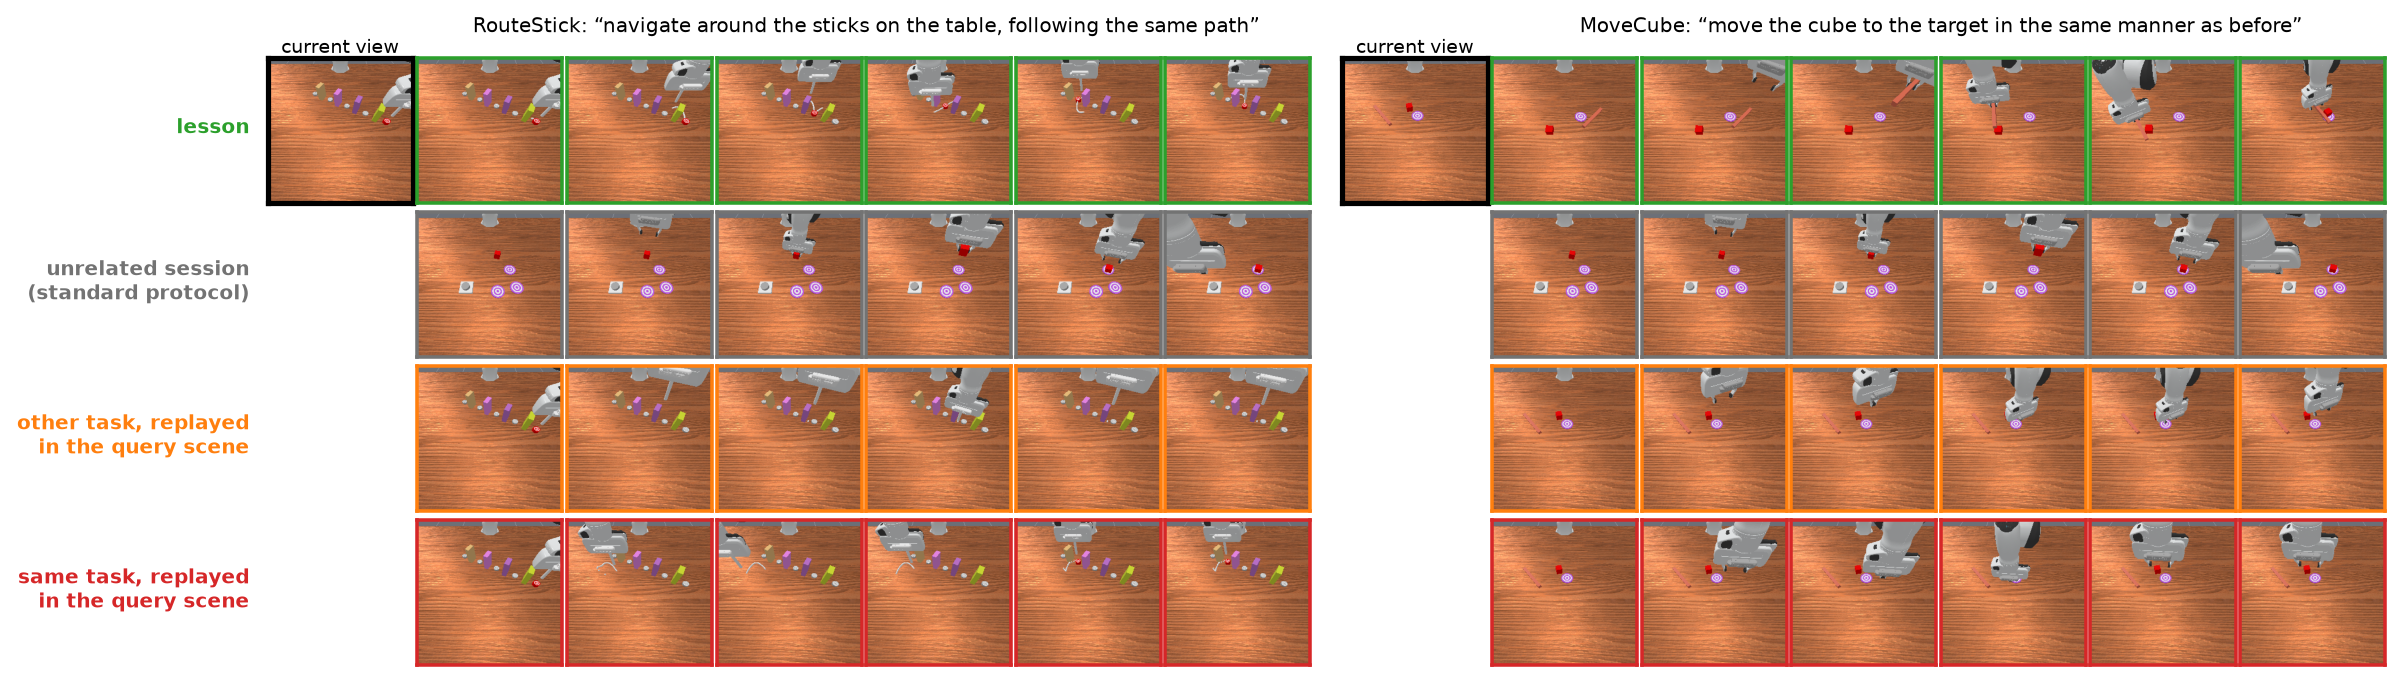
\includegraphics[width=\linewidth]{fig/qualitative.png}
\caption{Sessions of one test episode per task: six evenly spaced frames of the lesson, of an unrelated session (standard protocol), of a replay of another task recorded in the query scene (hard condition) and of a replay of the same task recorded in the query scene (same-task competitors). Black border: the view at the start of execution. Closed-loop success for the last row's condition: instruction router $.44$ (RouteStick) and $.48$ (MoveCube) against $.68$ and $.82$ with oracle routing.}
\label{fig:qual}
\end{figure}

\textbf{The manager, step by step.} Fig.~\ref{fig:algo} states the label-free manager used for the instruction-router rows.

\begin{figure}[h]
\centering\small
\fbox{\parbox{0.94\linewidth}{
\textbf{Input:} buffer frames $0..T$ with session boundaries; start $H$ of the current episode; instruction $g$; budget $B{=}32$; image and text encoders $\phi,\psi$ of a frozen SigLIP model; gate margin $\delta{=}.03$.\\[2pt]
\textbf{Once per episode (routing).}\\
\hspace*{1em}1. For each stored session $s$:\\
\hspace*{2.2em}$\mathrm{scene}_s=\max_{f\in s}\cos(\phi(f),\phi(o_H))$,\quad $\mathrm{text}_s=\max_{f\in s}\cos(\phi(f),\psi(g))$.\\
\hspace*{1em}2. Candidates $C=\{s:\mathrm{scene}_s\ge\max_{s'}\mathrm{scene}_{s'}-\delta\}$;\\
\hspace*{2.2em}$s^\star=\arg\max_{s\in C}\mathrm{text}_s$, with frames $[a,b)$ and $D=b-a$.\\[2pt]
\textbf{Every step (allocation and positions).}\\
\hspace*{1em}3. Select $B$ indices evenly over the concatenation of $[a,b)$ and $[H,T]$ (all of them if fewer than $B$).\\
\hspace*{1em}4. Re-index: a selected frame $i$ gets time position $i-a$ if $i<b$, and $D+(i-H)$ otherwise.\\
\hspace*{1em}5. Run the frozen policy on the selected frames at these positions.
}}
\caption{The label-free manager (instruction router + even comb + re-indexing). Steps 3--5 alone, with $s^\star$ given, are the lesson oracle; replacing steps 1--2 by per-step cosine similarity on the policy's own features gives retrieval + re-index.}
\label{fig:algo}
\end{figure}

\textbf{Intervals for the main tables.} Table~\ref{tab:ci} gives the paired differences behind Tables~\ref{tab:general} and~\ref{tab:hardstats} with their intervals.

\begin{table}[h]
\centering\small
\caption{Paired differences in success with Bonett--Price 95\% intervals ($n{=}50$ common episodes). ``Fix'': retrieval + re-index; ``router'': the label-free instruction router; hard-condition $k{=}0$ cells as in Table~\ref{tab:hardstats}.}
\label{tab:ci}
\setlength{\tabcolsep}{5pt}
\input{\ctrlroot ci_table}
\end{table}
